\documentclass[11pt,a4paper]{article}
\usepackage[utf8]{inputenc}
\usepackage[T1]{fontenc}
\usepackage{amsfonts}
\usepackage[french]{babel}
\frenchbsetup{StandardLists=true} % à inclure si on utilise \usepackage[francais]{babel}
\usepackage{enumitem}
\usepackage{amssymb}
\usepackage{amsmath}
\usepackage[left=2cm,right=2cm,top=2cm,bottom=2cm]{geometry}
\usepackage{multirow}
\usepackage[dvipsnames]{xcolor}

\usepackage[T1]{fontenc}
\usepackage{fouriernc}
\usepackage{graphicx}
\usepackage{colortbl}

\usepackage{setspace}
\singlespacing

\usepackage{pstricks}
\usepackage{xkeyval}
\usepackage{pst-labo}


\usepackage{multicol}
\usepackage{caption}
\usepackage{fancyhdr}
\pagestyle{fancy}
\renewcommand\headrulewidth{1pt}
\fancyhead[L]{Lycée Denis Diderot }
\fancyhead[R]{Classe de 1 Bac Pro }
\setcounter{page}{5}\fancyfoot[C]{page \thepage}
\fancyfoot[R]{Année 2024-2025}
\fancyfoot[L]{Alexis RUIZ}
\usepackage{multirow,tabularx,booktabs}
\newcommand{\cadreblanc}[1]{%
\medskip\framebox[\linewidth][c]{%
\rule{0mm}{#1mm}}\par
\medskip}

\usepackage{chemist} %chimie
\usepackage{awesomebox}
\setlength{\aweboxvskip}{0mm}
\usepackage{pifont}
\usepackage{chemmacros}
\chemsetup{modules=all}
\setlength{\columnseprule}{.25mm}

\renewcommand{\arraystretch}{2}
\newcolumntype{C}[1]{>{\centering\arraybackslash }b{#1}}


\newcommand{\code}{\awesomebox[black]{2pt}{

\includegraphics[scale=0.15]{../Chapitre 1 - Energie et puissance électrique/images/frame.png}
}{black}}



\newcommand{\defconclusion}{\awesomebox[black]{2pt}{\rotatebox{90}{\Large{\textbf{Conclusion}}}}{black}}


  \newenvironment{itemize*}%  % listes compactes
    {\begin{itemize}%
      \setlength{\itemsep}{0pt}%
      \setlength{\parskip}{0pt}}%
    {\end{itemize}}


\frenchbsetup{StandardLists=true}
\newlist{fleche}{itemize}{1}
\setlist[fleche]{label=\ding{220},font=\color{orange}}


\usepackage[tikz]{bclogo} 

\newcommand{\ctext}[1]
{\begin{bclogo}[couleur = white,logo= , arrondi = 0.1,barre=none]
{}
\vspace{-8mm}
~~
\textcolor{red}{#1}
~~
\end{bclogo}}

%%%%%%%%%%%%%%%%%%%%%%%%%%%%%%%%%%%%%%%%%%%%%%%%%%%%%%%%%%%



\begin{document}


\begin{center}
 \LARGE{COURS - Solution aqueuse } \\[3mm]
\end{center}


\normalsize

\hrule\
\\[0,5cm]


\fcolorbox{black}{white}{\textbf{\ding{202} Concentration en quantité de matière}}\\
\vspace{-3mm}

\begin{fleche}
\item \textbf{Quantité de matière}




\ctext{La quantité de matière $n$ est utilisée en chimie pour compter les atomes, les ions ou les molécules par "paquets" de $6,02 \times 10^{23}$. Son unité est la mole , symbole : mol.  }

\vspace{-5mm}

\begin{center}
\fbox{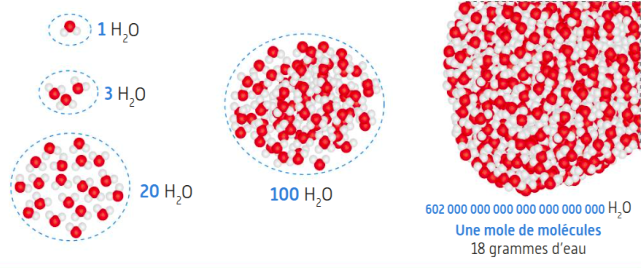
\includegraphics[scale=0.5]{images/Cours1.png}}
\end{center}

\item \textbf{Masse molaire}
\vspace{-3mm}
\begin{itemize}[label=\textbullet, font=\LARGE \color{black}]
\item 
\noindent% 
\begin{minipage}{.58\textwidth}%
\ctext{La masse molaire $M$, en g/mol, d'une espèce chimique  est la masse d'une mole de cette espèce. \\
\begin{center}
    $M = \dfrac{m}{n}$ d'où $n = \dfrac{m}{M}$
\end{center}
La classification périodique des éléments précise les différentes masses molaires atomiques. 
}
\end{minipage}% 
\hfill
\begin{minipage}{.27\textwidth}%
\fbox{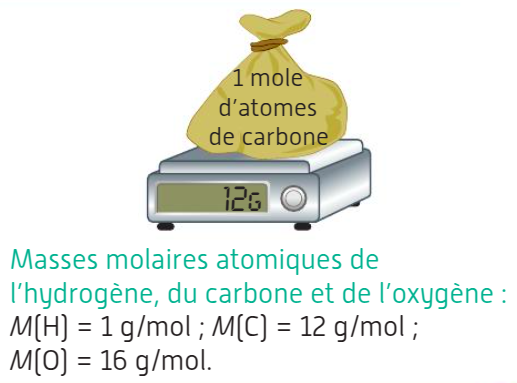
\includegraphics[width=\textwidth]{images/Cours2.png}}
\end{minipage}%
\item 
\begin{minipage}{.9\textwidth}%
\ctext{Dans le cas d'une molécules ont parle de masse molaire moléculaire (en g/mol). C'est la somme des masses molaires atomiques multiplié par le nombre d'atomes dans la molécule. \\[3mm]
Exemple : Pour le saccharose de formule \chemform{C_{12}H_{22}O_{11}}
\begin{center}
M(\chemform{C_{12}H_{22}O_{11}} = 12 $\times $ M(C) + 22 $\times$ M(H) + 11 $\times$ M(O)
\end{center}
\vspace{-3mm}
}
\end{minipage}
\end{itemize}

\item \textbf{Concentration en quantité de matière}
\vspace{-5mm}
\begin{itemize}
    \item 
    \begin{minipage}{.9\textwidth}%
    \ctext{Lorsque l'on dissout un corps (le \textbf{soluté}) dans un liquide (le \textbf{solvant}, le mélange homogène qu'il est résulte est une \textbf{solution}. Si le solvant est de l'eau, la solution est dite \textbf{aqueuse}. }

    \end{minipage}

    \item 
    \noindent
    \begin{minipage}{.72\textwidth}%
    \ctext{
    La concentration en quantité de matière C (en mol/L) d'une espèce chimique, appelé concentration molaire, est la quantité de matière de cette espèce dissoute dans un litre de solution aqueuse. 
    }
    \end{minipage}
    \hfill
\begin{minipage}{.15\textwidth}%
\ctext{$C=\dfrac{n}{V}$}
\end{minipage}%
    \vspace{-2mm}
        \item 
    \noindent
    \begin{minipage}{.72\textwidth}%
    \ctext{
    La concentration en masse \chemform{C_m} en g/L d'une espèce chimique est définie par : 
    }
    \end{minipage}
    \hfill
\begin{minipage}{.15\textwidth}%
\ctext{$C_m=\dfrac{m}{V}$}
\end{minipage}%

\end{itemize}

\end{fleche}
\end{document}